\appendix

\chapter{Spectrogram Examples}
\label{appx:spectra}

$Revision: 1.14 $

As produced by the \api{Spectrogram} class.

\begin{figure}[h]
	\centering
	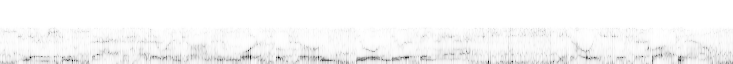
\includegraphics[width=500pt]{../graphics/lpc_spectrograms/ian15_wav.png}
	\caption{LPC spectrogram obtained for ian15.wav}
	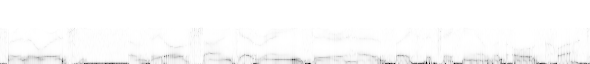
\includegraphics[width=500pt]{../graphics/lpc_spectrograms/graham13_wav.png}
	\caption{LPC spectrogram obtained for \file{graham13.wav}}
\end{figure}

%%%%%%%%%%%%%%%%%%%%%%%%%%%%%%%%%%%%%%%%%%%%%%%%%%

\chapter{MARF Source Code}

You can download
the code from \verb+<http://marf.sourceforge.net>+, specifically:

\begin{itemize}
	\item The latest unstable version:\\\verb+<http://marf.sourceforge.net/marf.tar.gz>+
	\item Browse code and revision history online:\\\verb+<http://cvs.sourceforge.net/cgi-bin/viewcvs.cgi/marf/>+
\end{itemize}

API documentation in the HTML format can be found in the documentation
distribution, or for the latest version please consult:
\verb+<http://marf.sourceforge.net/api/>+. If you want to participate
in development, there is a developers version of the API:
\verb+<http://marf.sourceforge.net/api-dev/>+, which includes
all the private constructs into the docs as well.

The current development version can also be retrieved via \tool{CVS}. The
process outlined in \xa{appx:cvs}.

\clearpage

%%%%%%%%%%%%%%%%%%%%%%%%%%%%%%%%%%%%%%%%%%%%%%%%%%

\chapter{The CVS Repository}
\label{appx:cvs}

The {\marf} source code is stored and managed using the
CVS code management system at SourceForge.
Anonymous CVS
is available to pull the CVS code tree from the
{\marf} package to your local machine.

\section{Getting The Source Via Anonymous CVS}

If you would like to keep up with the current sources on a regular
basis, you can fetch them from SourceForge's CVS server
and then use CVS to
retrieve updates from time to time.

\begin{itemize}
\item
     You will need a local copy of CVS
     (Concurrent Version Control System), which you can get from
     \verb+<http://www.cvshome.org/>+ or
     any GNU software archive site. There is also WinCVS and
     CVS mode built in JBulider if you plan to use these products
     on Win32 platforms.

\item
     Do an initial login to the CVS server:

\begin{verbatim}
cvs -d:pserver:anonymous@marf.cvs.sourceforge.net:/cvsroot/marf login
\end{verbatim}

     You will be prompted for a password; just press ENTER.
     You should only need to do this once, since the password will be
     saved in \verb+.cvspass+ in your home directory.

\item
     Fetch the {\marf} sources:

\begin{verbatim}
cvs -z3 -d:pserver:anonymous@marf.cvs.sourceforge.net:/cvsroot/marf co -P marf
\end{verbatim}

     which installs the {\marf} sources into a
     subdirectory \verb+marf+
     of the directory you are currently in.

     If you'd like to download sample applications which use {\marf}:

\begin{verbatim}
cvs -z3 -d:pserver:anonymous@marf.cvs.sourceforge.net:/cvsroot/marf co -P apps
\end{verbatim}


\item
     Whenever you want to update to the latest CVS sources,
     \verb+cd+ into
     the \verb+marf+ or \verb+apps+ subdirectories, and issue

\begin{verbatim}
cvs -z3 update -d -P
\end{verbatim}

     This will fetch only the changes since the last time you updated.

\item
     You can save yourself some typing by making a file \verb+.cvsrc+
     in your home directory that contains

\begin{verbatim}
cvs -z3
update -d -P
\end{verbatim}

     This supplies the \verb+-z3+ option to all \verb+cvs+ commands, and the
     \verb+-d+ and \verb+-P+ options to \verb+cvs update+.  Then you just have
     to say

\begin{verbatim}
cvs update
\end{verbatim}

     to update your files.

\end{itemize}


%%%%%%%%%%%%%%%%%%%%%%%%%%%%%%%%%%%%%%%%%%%%%%%%%%

\chapter{\api{SpeakerIdentApp} and \api{SpeakersIdentDb} Source Code}

\section{\texttt{SpeakerIdentApp.java}}

\vspace{15pt}
\hrule
{\scriptsize \input{SpeakerIdentApp}}
\hrule
\vspace{15pt}

\section{\texttt{SpeakersIdentDb.java}}

\vspace{15pt}
\hrule
{\scriptsize \input{SpeakersIdentDb}}
\hrule
\vspace{15pt}

\clearpage

%%%%%%%%%%%%%%%%%%%%%%%%%%%%%%%%%%%%%%%%%%%%%%%%%%

\chapter{TODO}
\label{appx:todo}

\vspace{15pt}
\hrule
{\scriptsize \input{TODO}}
\hrule
\vspace{15pt}

% EOF
